\documentclass[main.tex]{subfiles} % Subfile-Class


% ============================================================================== %
%                            Subfile document                                    %
% ============================================================================== %

\begin{document}

% Template

\subsection{Projektplanung}

Das Projekt wird in Sprints geplant. Ein Sprint dauert jeweils 2 Wochen, sodass
im Laufe des Semesters 7 Sprints entstehen. Für die einzelnen Sprints sind die
wichtigen Meilensteine, die Abgaben, bereits im Voraus eingeplant. Wichtige
Tätigkeiten, die eben in den entsprechenden Sprints stattfinden sollen, sind
ebenfalls im voraus bereits im Projektplan eingetragen. So ist immer klar,
welches Ziel zum Ende des Sprints erreicht werden soll.

Eine detaillierte Planung findet immer zu Sprint-Beginn statt - bei dem offene
Aufgaben entsprechend im Team verteilt werden. Diese Planung lebt und wird
laufend korrigiert dadurch, dass jeweils freitags in der Diskussionsrunde der
aktuelle Stand abgeholt, sowie gegebenenfalls Korrekturen an dieser Planung
vorgenommen werden.

Meetings innerhalb des Teams finden regelmässig einmal pro Woche, jeweils am
Freitag, statt. In dieser Gesprächsrunde werden zuerst die abgeschlossenen
Tasks besprochen, bevor im Anschluss eventuelle Knackpunkte im Team besprochen
werden können. So weiss jeder, woran der jeweils andere aktuell am Arbeiten ist
und es wird darüber hinaus eine Plattform geboten, Ideen und Anmerkungen aus
anderen Fachbereichen einfliessen zu lassen sowie Abhängigkeiten frühzeitig zu
erkennen und Teilentwicklungen aufeinander anzupassen.

\subsubsection*{Planungstool}
Das Projekt ist mit dem \textit{GitHub Projects} Tool geplant. Dieses Tool stellt im Wesentlichen
ein Kanban-Board dar, welches mit den vielen individuellen Optionen eine feine
Abstimmung auf verschiedene Projekte bietet.

Es ist für jedes Team-Mitglied eine Übersicht über den Gesamt-Backlog und eine
Ansicht für den individuellen Backlog eingerichtet. Die Ansicht
\textit{Roadmap} bietet eine Darstellung aller Tasks auf einem Zeitstrahl.
Grundsätzlich könnte zu jedem Issue gleich auch Dokumentation in Form von
Kommentaren geschrieben werden. In dieser Zusammenarbeit aber wird allerdings
in einem separaten Projektordner dokumentiert.
Abbildung~\ref{fig:GitHubProjectsTool} zeigt die verschiedenen Menüs sowie das
eingerichtete Kanban-Board für das Projektteam.

\begin{figure}[h!]
    \centering
    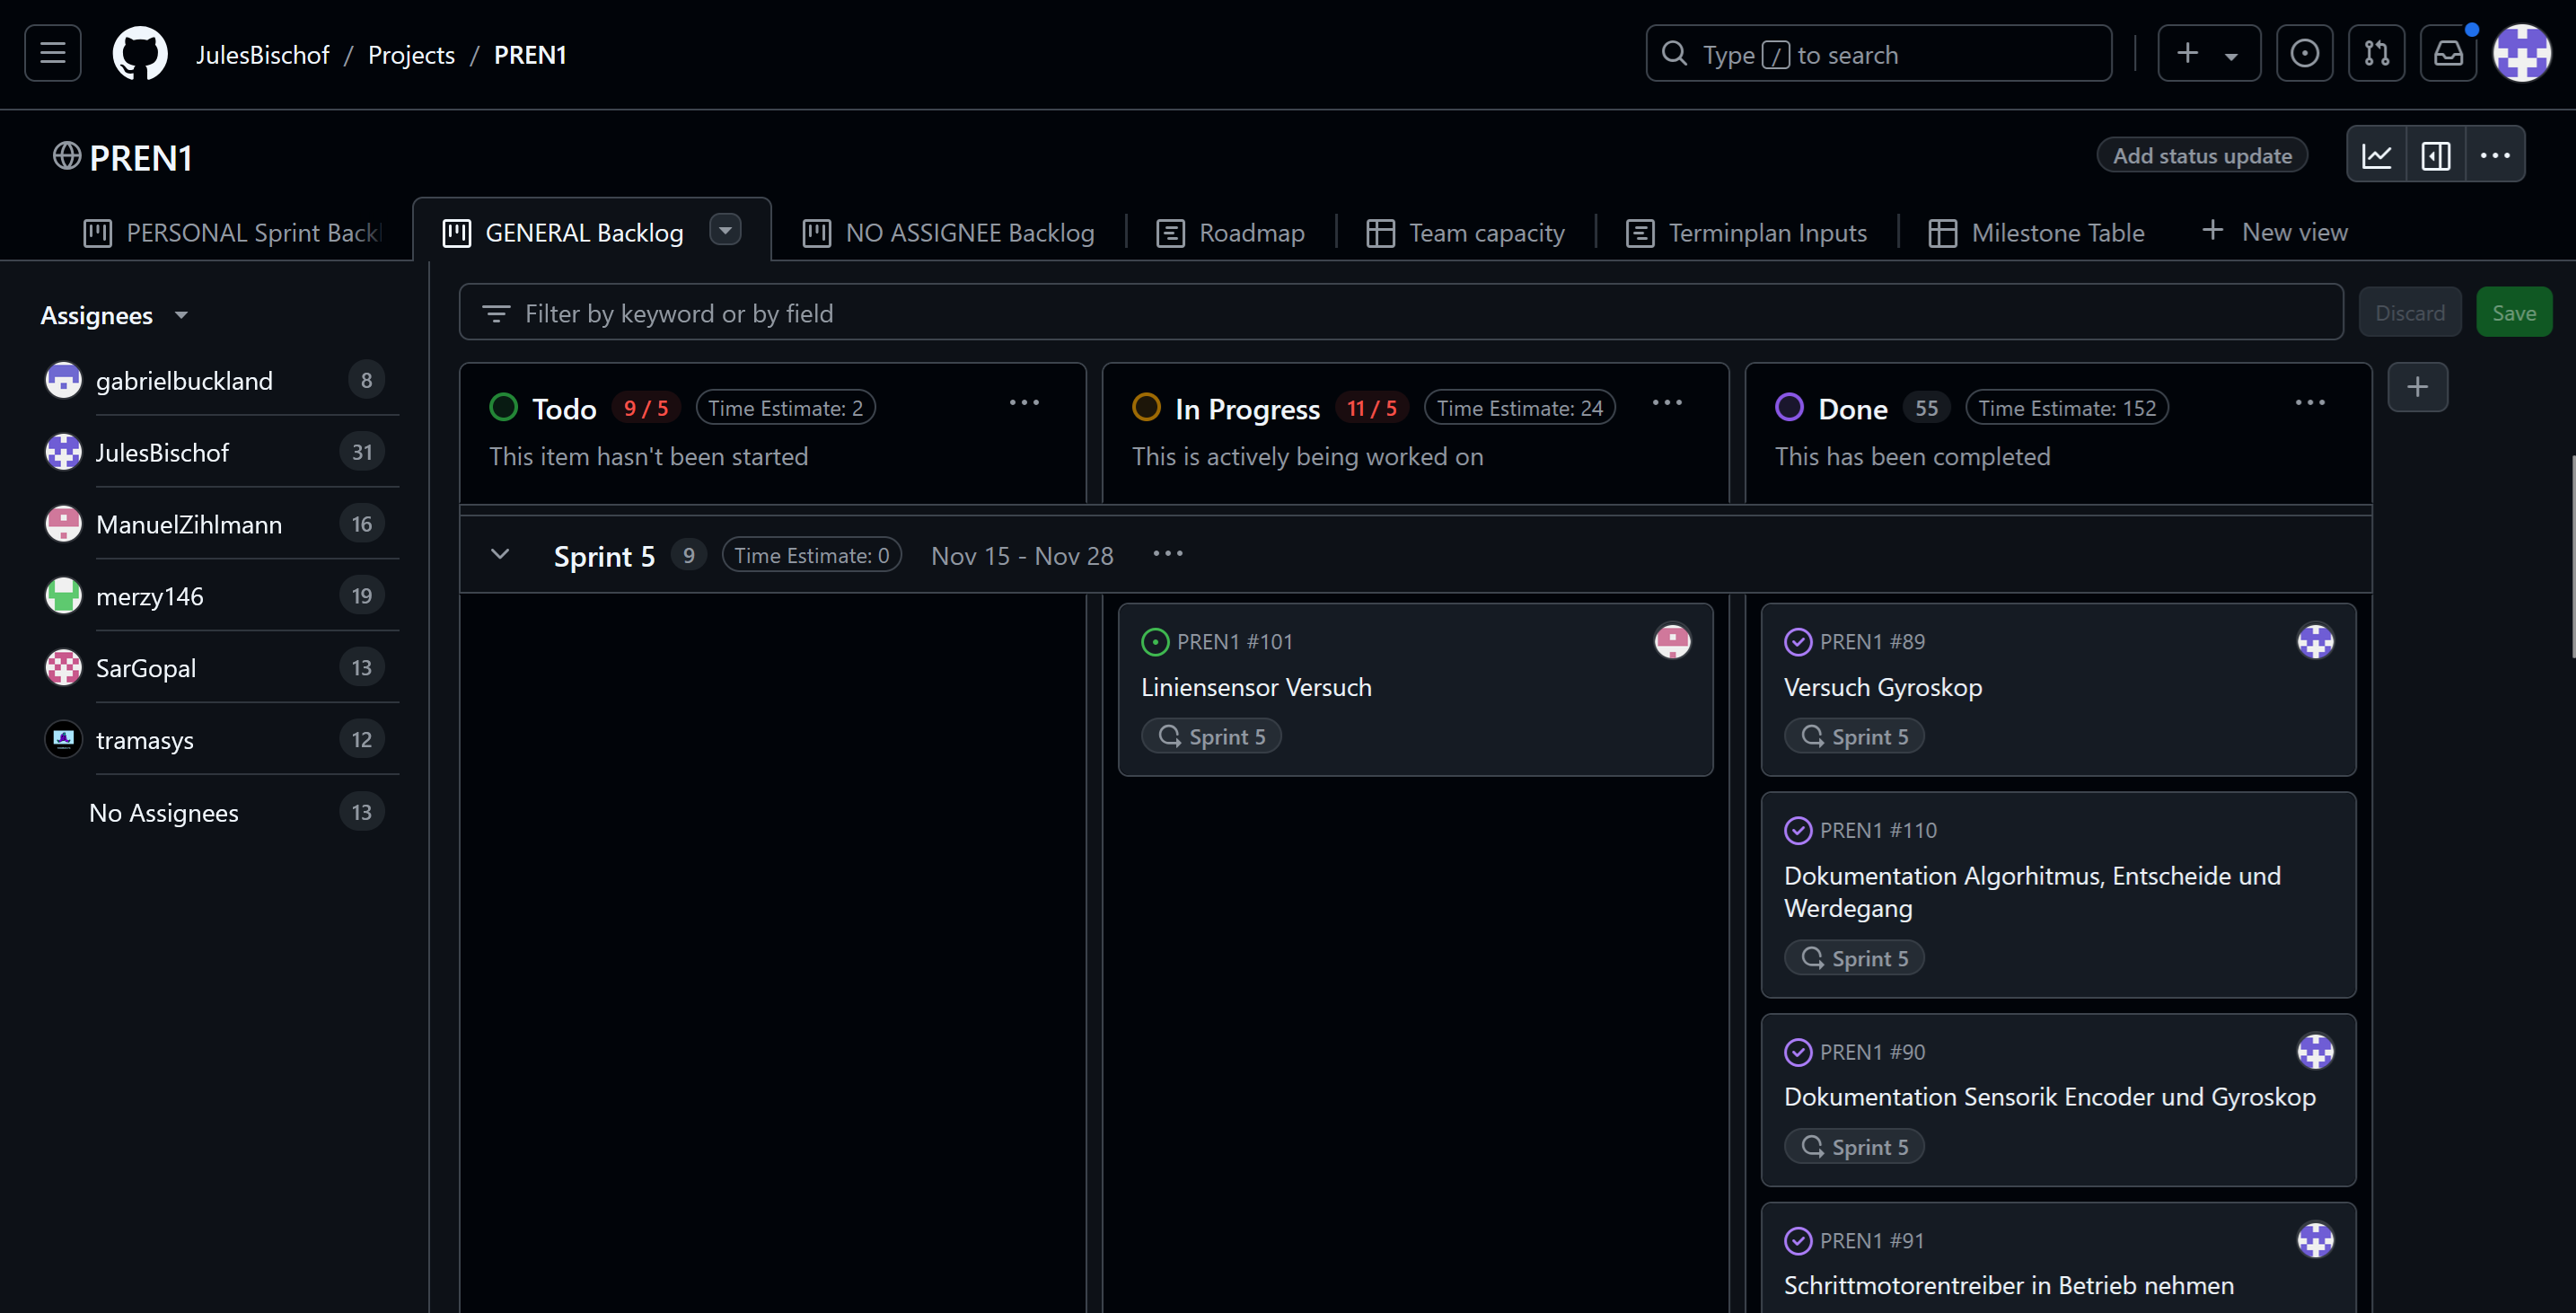
\includegraphics[page=1, width=1\textwidth]{./fig_Projektmanagement/Ansicht_GitHubProjects.png}
    \caption{GitHub Projects Tool}\label{fig:GitHubProjectsTool}
\end{figure}

\subsubsection*{Datenmanagement}
Es ist ein Projektordner eingerichtet, in welchem jedes Team-Mitglied seine Arbeit ablegen kann. Zugriff darauf
haben die Team-Mitglieder via \textit{OneDrive}.
Dabei gibt es für die Disziplinen Elektronik sowie Mechanik jeweils eigene Ordner, in denen Konstruktionsdaten,
CAD-Files oder etwa Bauteilauslegungen und PCB-Planungen abgelegt werden. Die Dokumentation
selbst wird in einem eigens dafür eingerichteten \textit{git Repository} geführt und versioniert.
Dadurch wird ermöglicht, dass jedes Team-Mitglied zur gleichen Zeit an der in \LaTeX geschriebenen
Dokumentation weiterarbeiten kann.

Der Teamleiter erstellt zu jedem Meilenstein bereits frühzeitig eine Vorlage
mit allen geforderten Unterdateien in Form einer Disposition. Jedes geforderte
Kapitel wird dabei durch eine eigene Unterdatei repräsentiert. So kommt es nur
sehr unwahrscheinlich zu Merge-Konflikten innerhalb des Repositorys und es kann
mit \textit{Trunk-based development} gearbeitet werden - was den Einstieg in
\textit{git} für unerfahrene Mitglieder vereinfacht.

\end{document}
